In this section we make a change of coordinates which covers the maximally extended black hole solution. This two sided hot phase solution is considered to have a dual CFT sitting on its boundary in the pure thermofield double state. We then make another change of coordinates to draw Penrose diagrams. As the second spatial dimension $x_j$ features walls, we make $3$ dimensional Penrose diagrams of the hot phase to make a clear representation of the geometry. We follow mainly the analysis of \cite{Ba_ados_1993}.

\section{Kruskal-Szekeres coordinates}

As in the Schwarzschild solution, the horizon is only a coordinate singularity and can be removed by a change of coordinates. One can verify this by checking that the value of all the possible curvature invariants as we approach the horizon remain finite. This is simply the manifestation of the equivalence principal stating that a free observer falling towards $r=0$ should not feel any difference as they cross the horizon. The Kruskal-Szekeres coordinates are such set of coordinates that remove this singularity and cover the maximally extended black hole. They are related to $(t,r)$ by
\begin{subequations}
    \label{Kruskal coord}
    \begin{align}
        u = \sqrt{\frac{r-r_h}{r+r_h}}\cosh{\frac{r_ht}{\ell}},\label{kruskal u}\\
        v = \sqrt{\frac{r-r_h}{r+r_h}}\sinh{\frac{r_ht}{\ell}}.\label{kruskal v}
    \end{align}
\end{subequations}

This change of coordinates results in the following metric,
\begin{equation}\label{kruskal metric}
    \text{d}s^2=\Omega^2(u,v)\left(\text{d}u^2-\text{d}v^2+M\frac{\left(u^2-v^2+1\right)^2}{4}\text{d}x^2\right),
\end{equation}
where the conformal factor is $\Omega^2(u,v)=\frac{(r+r_h)^2}{M}$. Or in the new coordinates,
\begin{equation}
    \Omega^2(u,v)=\frac{4\ell^2}{\left(u^2-v^2-1\right)^2}.
\end{equation}
The K-S metric originally covers the region $r>r_h$ but it can be analytically continued to the region $0<r<r_h$. The coordinate change (\ref{Kruskal coord}) concerns the region outside the horizon. We can clearly see that these coordinates are well-behaved as we are traversing the horizon except at the physical singularity $r=0$. 

\section{3 dimensional Penrose diagram}

There is a better way to represent a black hole spacetime where we can include infinite points. To do this, we make a conformal compactification in such a way that all points at $\infty$ in the original metric are at finite affine parameter in the new metric. For example, for a  2 dimensional Minkowski space-time, where the metric has the form $ds^2= -dt^2 + dx^2$ and $(x,t)\in(-\infty,\infty)$, we can find new coordinates $\left(\psi,\xi\right)\in\left(-\pi,\pi\right)$ such that the new metric is written like 
\begin{equation}
    ds^2 = \Lambda^2\left(\psi,\xi\right)\left(-d\psi^2+d\xi^2\right).
\end{equation}
The conformal coefficient $\Lambda$ diverges at $\pi$ and $-\pi$.

One can derive in the same way a coordinate system for BTZ black holes. This is done by the following change of coordinates
\begin{subequations}
\label{Penrose coord}
\begin{align}
     u + v = \tan\frac{p+q}{2},\label{Perose +}\\
     u - v = \tan\frac{p-q}{2},\label{Penrose -}
\end{align}
\end{subequations}
where $p,q\in[-\frac{\pi}{2},\frac{\pi}{2})$.

The metric \ref{kruskal metric} becomes,
\begin{equation}\label{metricdial Penrose}
    \text{d}s^2=\frac{\ell^2}{\cos^2(p)}\left(\text{d}p^2-\text{d}q^2+M\cos^2(q)\text{d}x^2\right).
\end{equation}


Penrose diagrams help represent causal relations between different spacetime points with conformal compactification. The 2 dimensional Penrose diagram was represented in figure \ref{Penrose diagram thermofield double}.

\begin{figure}
    \centering
    \begin{subfigure}[b]{0.45\textwidth}
        \centering
        \includegraphics[width=\textwidth]{figures/pen3dred.png}
        \caption{}
        \label{penrosered}
    \end{subfigure}
    \hfill
    \begin{subfigure}[b]{0.45\textwidth}
        \centering
        \includegraphics[width=\textwidth]{figures/pen3dblue.png}
        \caption{}
        \label{penroseblue}
    \end{subfigure}
    \caption{3 dimensional Penrose diagrams of the two slices. The two walls diverge at the singularity. While the red slice's walls diverge in different directions, the blue ones diverge towards each other in the $x$ direction which leads to a wall collision near the singularity.}
    \label{penrose3d}
\end{figure}

Since we have an $x$ coordinate that features walls in the hot phase discussed earlier, we would like to add the $x$ axis to the Penrose picture. This will result in a sort of 3 dimensional plots. The wall solution computed in chapter \ref{section 5} can be given in terms of the ($p,q$) coordinates. Using equation (\ref{mysolved}), the wall equation becomes
\begin{equation}\label{l7it dial Penrose}
    \alpha_j(p_j,q_j) = \frac{1}{2\pi T}\tanh^{-1}\left(\frac{\ell_j\left(\lambda^2+\epsilon_j{\lambda_0}^2\right)}{2\lambda}\frac{1}{\sqrt{a_j\left(\frac{\cos^2(q_j)}{\cos^2(p_j)}-1\right)+1}}\right) + \frac{L_j}{2},
\end{equation}
where $\epsilon_j=\delta_{j,1}-\delta_{j,2}$. The continuation of the wall solution behind the horizon diverges at the singularity. The two walls seem to collide before reaching this point. The 3D Penrose diagram is represented in \ref{penrose3d}.

We can see from the change of the coordinates (\ref{Penrose coord}) that:
\begin{itemize}
  \item The point $r\to\infty$ corresponds to the point $p=\pm\frac{\pi}{2}$,
  \item The point $r=0$ corresponds to the point $q=\pm\frac{\pi}{2}$,
  \item The point $r=r_h$ corresponds to the point $p=\pm q$.
\end{itemize}

\section{RT surfaces and Page curve}

We can derive a version of the information paradox in the case at hand. The double sided geometry computed in the previous section is dual to an ICFT in a pure state living on the double boundary $M\cup M'$ of fig. \ref{Penrose diagram thermofield double}.

We want to compute time dependant RT surfaces. This can be considered by taking the boundary region to sit in a constant $q$ slice. If we move the right side forward, while moving the left side downwards in the $q$ direction, it will leave the state of the system unchanged as it is an isometry. This can also be seen in the case of the thermofield double by evolving the purified state with respect to the Hamiltonian $H = H_1-H_2$, where $H_i$ is the Hamiltonian of the $j^\text{th}$ copy. However, we can move both sides in the upward direction of $q$. Computing RT surfaces in this case gives time dependant entropies.

The RT surfaces in question are those homologous to the double sided interval $\Tilde{A}=A\cup A'$, see fig. \ref{aua'}. There are two possible RT surfaces. The first one is composed of two symmetric surfaces $m(A)$ and $m(A')$ respectively homologous to $A$ and $A'$. The second one is a surface linking a point in $\partial A$ to a point in $\partial A'$ and its symmetric surface linking the two other boundary points. The schematic RT surfaces are represented in fig. \ref{aua'}.

\begin{figure}
    \centering
    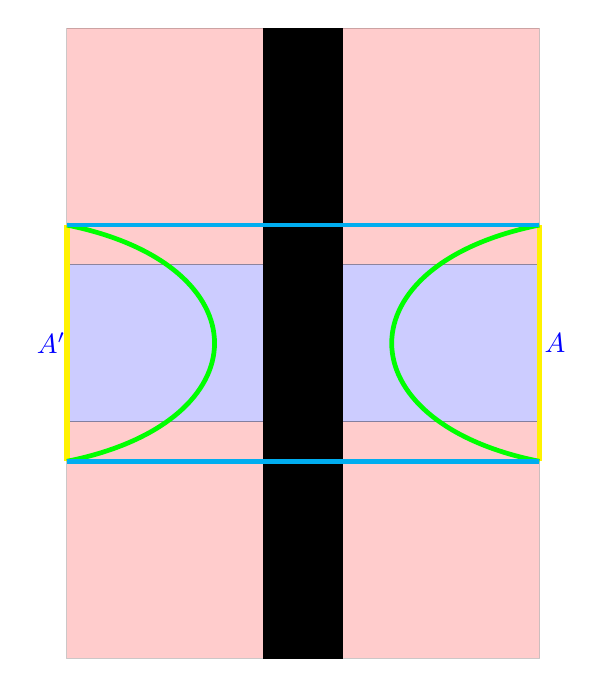
\begin{tikzpicture}
        \draw[black, fill=red, opacity=0.2] (-3,1) -- (3,1) -- (3,4) -- (-3,4) -- (-3,1);
        \draw[black, fill=blue, opacity=0.2] (-3,1) -- (3,1) -- (3,-1) -- (-3,-1) -- (-3,1);
        \draw[black, fill=red, opacity=0.2] (-3,-1) -- (3,-1) -- (3,-4) -- (-3,-4) -- (-3,-1);
        \draw[fill=black] (-.5,4) -- (.5,4) --(.5,-4) -- (-.5,-4) -- (-.5,4);
        \draw[yellow, line width=2] (3,1.5) -- (3,-1.5);
        \draw[yellow, line width=2] (-3,1.5) -- (-3,-1.5);
        \draw[color=green,line width=.6mm] (3,1.5) .. controls (.5,1) and (.5,-1) .. (3,-1.5);
        \draw[color=green,line width=.6mm] (-3,1.5) .. controls (-.5,1) and (-.5,-1) .. (-3,-1.5);
        \draw[color=cyan,line width=.6mm] (3,1.5) -- (-3,1.5);
        \draw[color=cyan,line width=.6mm] (3,-1.5) -- (-3,-1.5);
        \draw[blue] node at (3.2,0){$A$};
        \draw[blue] node at (-3.2,0){$A'$};
    \end{tikzpicture}
    \caption{Representation of constant $q$ slice of the 3d Penrose diagram. The black stripe represents the horizon. At $q=0$ this stripe is a line. We have two possible RT surfaces represented in blue and green.}
    \label{aua'}
\end{figure}

The blue RT surface, in fig. \ref{aua'}, links two opposite points on the cutoff surface. These surfaces remain in the red slice for $\pi h>\beta$. This can be seen from eq. (\ref{l7it dial Penrose}), which shows that $x_i$ is a monotonic function of $p_i$ and $x_i(0)-x_i(\infty)\leq \beta/\pi$. Also, the symmetry of the geometry (\ref{metricdial Penrose}) with respect to $x_i$ requires that the blue geodesics are at constant $x_i$. This makes the time dependence of the metric (\ref{metricdial Penrose}) vanish. The blue RT surface is then computed as follows
\begin{align}\label{thela Lagrangian}
    L &= 2\ell_1\int\frac{\text{d}p_1}{\cos(p_1)}\\
    &= 4\ell_1\cdot\log\left(\tan(p_1)+\frac{1}{\cos(p_1)}\right)\bigg|_{p_{\epsilon}}
\end{align}
where the factor of 2 refers to having two similar RT surfaces and $p_\epsilon$ is the cutoff surface.

The time dependence of this geodesic comes from the non trivial cutoff surface ${p_{\epsilon(q_1)}}$. This cutoff surface is found from the Penrose change of coordinates by setting $r=1/\epsilon$. We find\footnote{see appendix \ref{appendix E} for detailed calculations},
\begin{equation}
    \cos({p_{\epsilon(q_1)}}) = \epsilon{r_h}_1\cos(q_1).
\end{equation}

\begin{figure}
    \centering
    \includegraphics[width=0.7\textwidth]{figures/Real_time_Page.png}
    \caption{The entropy $S$ of the boundary interval $\Tilde{A}$ given by equation (\ref{thats}). We see a rising entropy $S_1$ at the beginning, The growth is linear for $t\ll \beta$. The entropy growth stops  at $t\sim\frac{\beta S_2}{c_1}$ and takes the value $S_2$.}
    \label{the final Page curve}
\end{figure}

Putting all of this together, we find the length of the RT surface, as we expand around $\epsilon=0$, to be
\begin{equation}\label{c'est bon}
    S_1(q_1) = \frac{2}{3}c_1\log\left(\frac{\beta}{\pi\ell_1\epsilon}\frac{1}{\cos(q_1)}\right).
\end{equation}

This entropy is an increasing function of $q_1$. We would like to recover the real time dependence $t$. Using the change of coordinates (\ref{Penrose coord}), we find
\begin{equation}
    \cos^2(q_1)=\frac{1-\tanh^2(2\pi t/\beta)}{1-\epsilon^2{r_h_1}^2\tanh^2(2\pi t/\beta)}.
\end{equation}
This is shown in appendix \ref{appendix E}.
Putting this expression in (\ref{c'est bon}), we find
\begin{equation}
    S_1(t) = \frac{2}{3}c_1\log\left(\frac{\beta}{\pi\ell_1\epsilon}\cosh\left(\frac{2\pi t}{\beta}\right)\right).
\end{equation}

The plot of $S_1$ is represented in fig. \ref{the final Page curve}. After a few thermal times, the growth becomes linear with a slope given by the temperature of the black hole and the central charge,
\begin{equation}
    S_1(t) \rightarrow \frac{4\pi}{3}c_1\frac{t}{\beta} + ...,
\end{equation}
where the $...$ refer to some constant term including the UV divergence. The entropy growth would be a paradox if it went on for a long time. This is similar to the Hawking paradox, since the linear growth leads to an overfilling of the black hole
\begin{equation}
    S_1\left(t>t_\text{Page}\right)>2S_\text{BH}.
\end{equation}

There is still another RT surface homologous to $\Tilde{A}$, the green RT surface. We hope that this RT surface will make an end to the linear growth of the entropy at the Page time. It is composed of two symmetric surfaces, each living in one side of the double geometry. These geodesics are actually the same as that computed in eq. (\ref{S2}). Since the geometry is static in the original coordinates, the RT surfaces remain constant as time flows. The value of this entropy is then,
\begin{equation}
    S^*_2= \frac{c_1}{3}\log\left(\frac{\beta}{\pi\ell_1\epsilon}\cosh\left(\frac{\pi h}{\beta}+\tanh^{-1}Y\right)\right)+\frac{\pi c_2}{3\beta}L_2+\frac{c_2}{3}\tanh^{-1}X,
\end{equation}
where $X=\frac{\ell_2\left(\lambda^2-{\lambda_0}^2\right)}{2\lambda}$ and $Y=\frac{\ell_1\left(\lambda^2+{\lambda_0}^2\right)}{2\lambda}$. The full entropy is given by the minimum of the two expression
\begin{equation}\label{thats}
    S = \min\left \{S_1,S_2\right \}.
\end{equation}

We see that the entropy starts rising at first, until it reaches the constant value $S_2$ which saturates the entropy and remains constant for the rest of time. This entropy growth given by $S_1$ is similar to Hawking's information paradox since it surpasses the coarse grained entropy at the Page time. This infinite growth contradicts the finite number of states of the boundary QM system. We solve this paradox by means of the other RT surface $S_2$. We suspect that the result should remain the same in the case of multiple slices inside the blue slice as long as the their corresponding central charges remains larger than that of the exterior slice. Because of the symmetry (w.r.t x) of the BTZ geometry, the linear growth of the entropy in the hot phase is the same as the one in the normal BTZ phase without walls.


